%% LyX 2.3.7 created this file.  For more info, see http://www.lyx.org/.
%% Do not edit unless you really know what you are doing.
\documentclass[12pt,english]{article}
\usepackage[T1]{fontenc}
\usepackage[latin9]{inputenc}
\usepackage{geometry}
\geometry{verbose,tmargin=1in,bmargin=1in,lmargin=1in,rmargin=1in}
\usepackage{amsmath}
\usepackage{graphicx}
\usepackage{setspace}
\onehalfspacing

\makeatletter

%%%%%%%%%%%%%%%%%%%%%%%%%%%%%% LyX specific LaTeX commands.
%% Because html converters don't know tabularnewline
\providecommand{\tabularnewline}{\\}

\makeatother

\usepackage{babel}
\usepackage[style=authoryear,backend=bibtex]{biblatex}
\begin{document}
\begin{figure}
\caption{Lexis diagram(s) for completed cohort fertility (focal cohort = $c$)}
\label{fig-Lexis}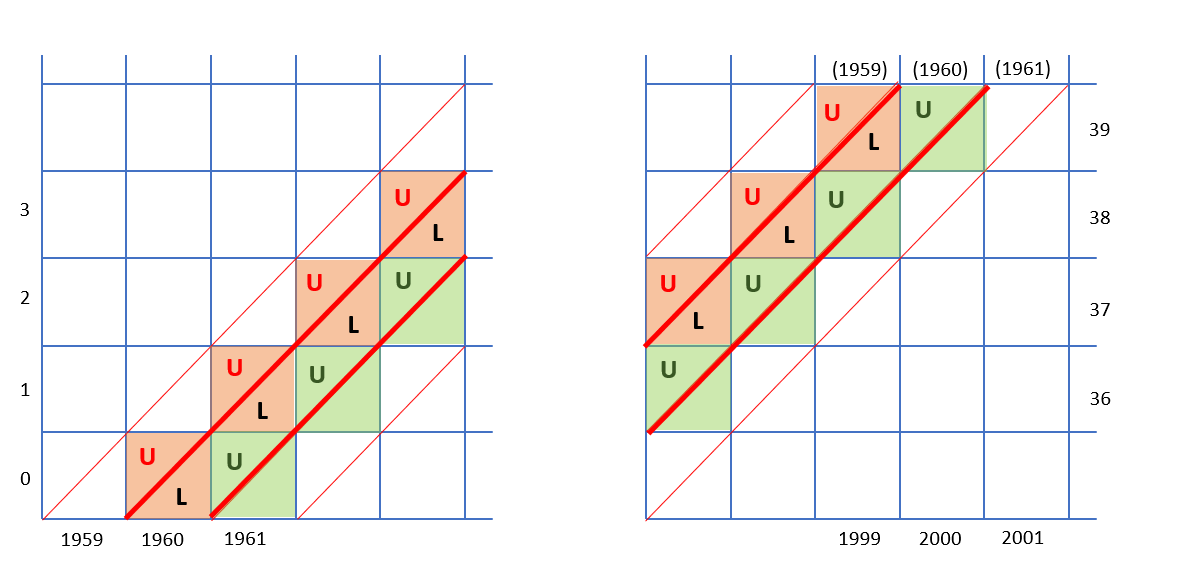
\includegraphics[width=0.9\textwidth,bb = 0 0 200 100, draft, type=eps]{pasted1.png}
\end{figure}

Consider an age-period Lexis grid as in Fig. \ref{fig-Lexis}, divided
into age-period-cohort triangles. Suppose that we are interested in
estimating the average completed fertility of the $N_{c}$ women born
in year $c$ when they reach exact age 40. Define $L_{xt}$ and $U_{xt}$
as the number of births that happen in the lower and upper triangles,
respectively, of the age-period square for age $x$, year $t$. If
there were no mortality before the highest age of childbearing, then
the sequence of single-year birth rates for cohort $c$ before exact
age 40 is
\[
\left(\frac{L_{0,c}+U_{0,c+1}}{N_{c}},\frac{L_{1,c+1}+U_{1,c+2}}{N_{c}},\ldots,\frac{L_{39,c+39}+U_{39,c+40}}{N_{c}}\right)
\]
and truc cohort completed fertility equals
\begin{align*}
F_{c}\, & =\,\sum_{x=0}^{39}\frac{L_{x,c+x}+U_{x,c+x+1}}{N_{c}}\\
 & =\,\frac{L_{c}^{\ast}+U_{c}^{\ast}}{N_{c}}
\end{align*}
where we subdivide the births by category of Lexis triangle (lower
or upper) and use {*} to indicate summation over ages.

If instead we sum the birth rates ``along the diagonal'' in age-period
cells {[}($0,c),(1,c+1)\ldots(39,c+39)${]} then we replace the ``upper''
cells for cohort $c$ with those from the previous cohort $c-1$,
and replace exposure with an average of cohort sizes $N_{c}$ and
$N_{c-1}$. If we sum these age-period rates over ages we produce
the \emph{AP-diagonal }estimate for completed fertility: 

\[
\hat{F}_{c}=\frac{U_{c-1}^{\ast}+L_{c}^{\ast}}{\tfrac{1}{2}(N_{c-1}+N_{c})}
\]


\subsection*{Simplifying Approximations}

In order to develop a simple expression for ``diagonal bias'' $\hat{F}_{c}-F_{c}$,
assume that
\begin{enumerate}
\item Mortality is negligible below the highest age of childbearing 
\item In a small neighborhood around our focal cohort $c$, cohort sizes
change multiplicatively: $N_{c}=KN_{c-1},\,N_{c+1}=KN_{c}$ 
\item In a small neighborhood around our focal cohort $c$, completed fertility
changes linearly: $\left(F_{c}-F_{c-1}\right)=\left(F_{c+1}-F_{c}\right)=\Delta$
\item Half of a cohort's lifetime births happen in lower Lexis triangles,
half in upper triangles: $L_{c}^{\ast}=U_{c}^{\ast}\approx\tfrac{1}{2}N_{c}F_{c}$
\end{enumerate}
Under these assumptions the AP-diagonal estimator for completed fertility
of the cohort born in year $c$ is 
\[
\hat{F}_{c}\approx\frac{\tfrac{1}{2}N_{c-1}F_{c-1}+\tfrac{1}{2}N_{c}F_{c}}{\tfrac{1}{2}(N_{c-1}+N_{c})}
\]
If cohort sizes around $c$ are changing multiplicatively with annual
multiplier $K$, this implies that 
\begin{align*}
\hat{F}_{c} & \approx\frac{\tfrac{1}{2}N_{c-1}F_{c-1}+\tfrac{1}{2}KN_{c-1}F_{c}}{\tfrac{1}{2}(N_{c-1}+K\cdot N_{c-1})}\\
 & =\frac{F_{c-1}+KF_{c}}{K+1}\\
 & =\left(\tfrac{1}{K+1}\right)F_{c-1}+\left(\tfrac{K}{K+1}\right)F_{c}
\end{align*}
That is, the AP-diagonal estimator is is approximately equal to a
weighted average of the previous and current cohort's completed fertility.
Rexpressing the AP-diagonal estimator in terms of cross-cohort changes
in completed fertility yields
\begin{align}
\hat{F}_{c} & =\,\left(\tfrac{1}{K+1}\right)\left(F_{c}-\Delta\right)+\left(\tfrac{K}{K+1}\right)F_{c}\label{eq:Fchat-bias}\\
 & =\,\underbrace{F_{c}}_{\text{true cohort value}}+\underbrace{\left(-\tfrac{\Delta}{K+1}\right)}_{\text{AP diagonal bias}}\nonumber 
\end{align}
From Eq. (\ref{eq:Fchat-bias}) we see that 
\begin{itemize}
\item regardless of cohort size differences, AP diagonal bias is negative
when completed fertility is rising with cohort birth year ($\Delta>0),$positive
when completed fertility is falling ($\Delta<0),$and zero when completed
fertility is unchanging ($\Delta=0$). 
\item AP diagonal bias is smaller in absolute value when cohort size is
increasing more quickly between consecutive birth years (larger $K$
implies bias closer to zero, because there is a higher weight on the
cohort of interest)
\end{itemize}

\subsection*{A better approximation: Averaging two AP diagonals}

Fig. \ref{fig-Lexis} shows that the AP-diagonal estimate $\hat{F}_{c}$
discards the ``U'' births from cohort $c$ and replaces them with
the ``U'' births from the previous cohort $c-1$. The$\hat{F}_{c}$
estimator is thus pulled toward the past, resulting in temporal bias
that can be magnified (or reduced) by cohort size differences. Intuitively,
we might be able to reduce temporal bias by using information from
birth cohorts born just before \emph{and just after }the cohort of
interest. This intuition is correct: we can produce a temporally more
symmetric estimate by combibing the biased AP diagonal estimators
for cohorts $c$ and $c+1$:
\[
\hat{F}_{c}=F_{c}-\frac{\Delta}{K+1}\qquad\text{and\ensuremath{\qquad\hat{F}_{c+1}=F_{c+1}-\frac{\Delta}{K+1}}}
\]

Define the \emph{AP2-diagonal} estimator
\[
\tilde{F}_{c}=\,\tfrac{1}{2}\hat{F}_{c}+\tfrac{1}{2}\hat{F}_{c+1}
\]
and note that 
\begin{align}
\tilde{F}_{c} & =\,\tfrac{1}{2}\left(F_{c}-\frac{\Delta}{K+1}\right)+\tfrac{1}{2}\left(F_{c+1}-\frac{\Delta}{K+1}\right)\nonumber \\
 & =\,\tfrac{1}{2}\left(F_{c}-\frac{\Delta}{K+1}\right)+\tfrac{1}{2}\left(F_{c}+\Delta-\frac{\Delta}{K+1}\right)\nonumber \\
 & =\,\underbrace{F_{c}}_{\text{true cohort value}}+\,\underbrace{\left[-\left(\frac{K-1}{2}\right)\left(\frac{\Delta}{K+1}\right)\right]}_{\text{AP2 diagonal bias}}\label{eq:Fctilde-bias}
\end{align}

The AP2 diagonal bias for $\tilde{F}_{c}$ in Eq. (\ref{eq:Fctilde-bias})
will almost always be much smaller than the AP diagonal bias for $\hat{F}_{c}$
in Eq. (\ref{eq:Fchat-bias}). Both bias terms contain $-\left(\tfrac{\Delta}{K+1}\right)$,
but for $\tilde{F}_{c}$ that term is multiplied by a small fraction,
rather than one. Table \ref{tab:compare-bias} shows illustrative
examples of biases for the two estimators, using a few represtentative
example values for $K$ and $\Delta$. When cohort fertility is changing
($\Delta\ne0$) the $\tilde{F}_{c}$ estimator has much lower bias
than $\hat{F}_{c}$.

\begin{table}
\caption{Comparative Bias of AP and AP2 estimates of Completed Cohort Fertility}

\begin{tabular}{|c|c|c|c|}
\hline 
 &  & \multicolumn{2}{c|}{Bias}\tabularnewline
\hline 
$K$ & $\Delta$ & $\hat{F_{c}}$(AP) & $\tilde{F}_{c}$ (AP2)\tabularnewline
\hline 
\hline 
0.9 & -.20 & +.1050 & +.0053\tabularnewline
\hline 
0.9 & 0 & 0 & 0\tabularnewline
\hline 
0.9 & +.20 & -.1050 & -.0053\tabularnewline
\hline 
1.0 & -.20 & +.1000 & 0\tabularnewline
\hline 
1.0 & 0 & 0 & 0\tabularnewline
\hline 
1.0 & +.20 & -.1000 & 0\tabularnewline
\hline 
1.1 & -.20 & +.0952 & -.0048\tabularnewline
\hline 
1.1 & 0 & 0 & 0\tabularnewline
\hline 
1.1 & +.20 & -.0952 & +.0048\tabularnewline
\hline 
\end{tabular}\label{tab:compare-bias}
\end{table}


\subsection*{Comparisons with the Japanese Fertility Data from van Raalte et al. }

\begin{figure}
\caption{JPN}

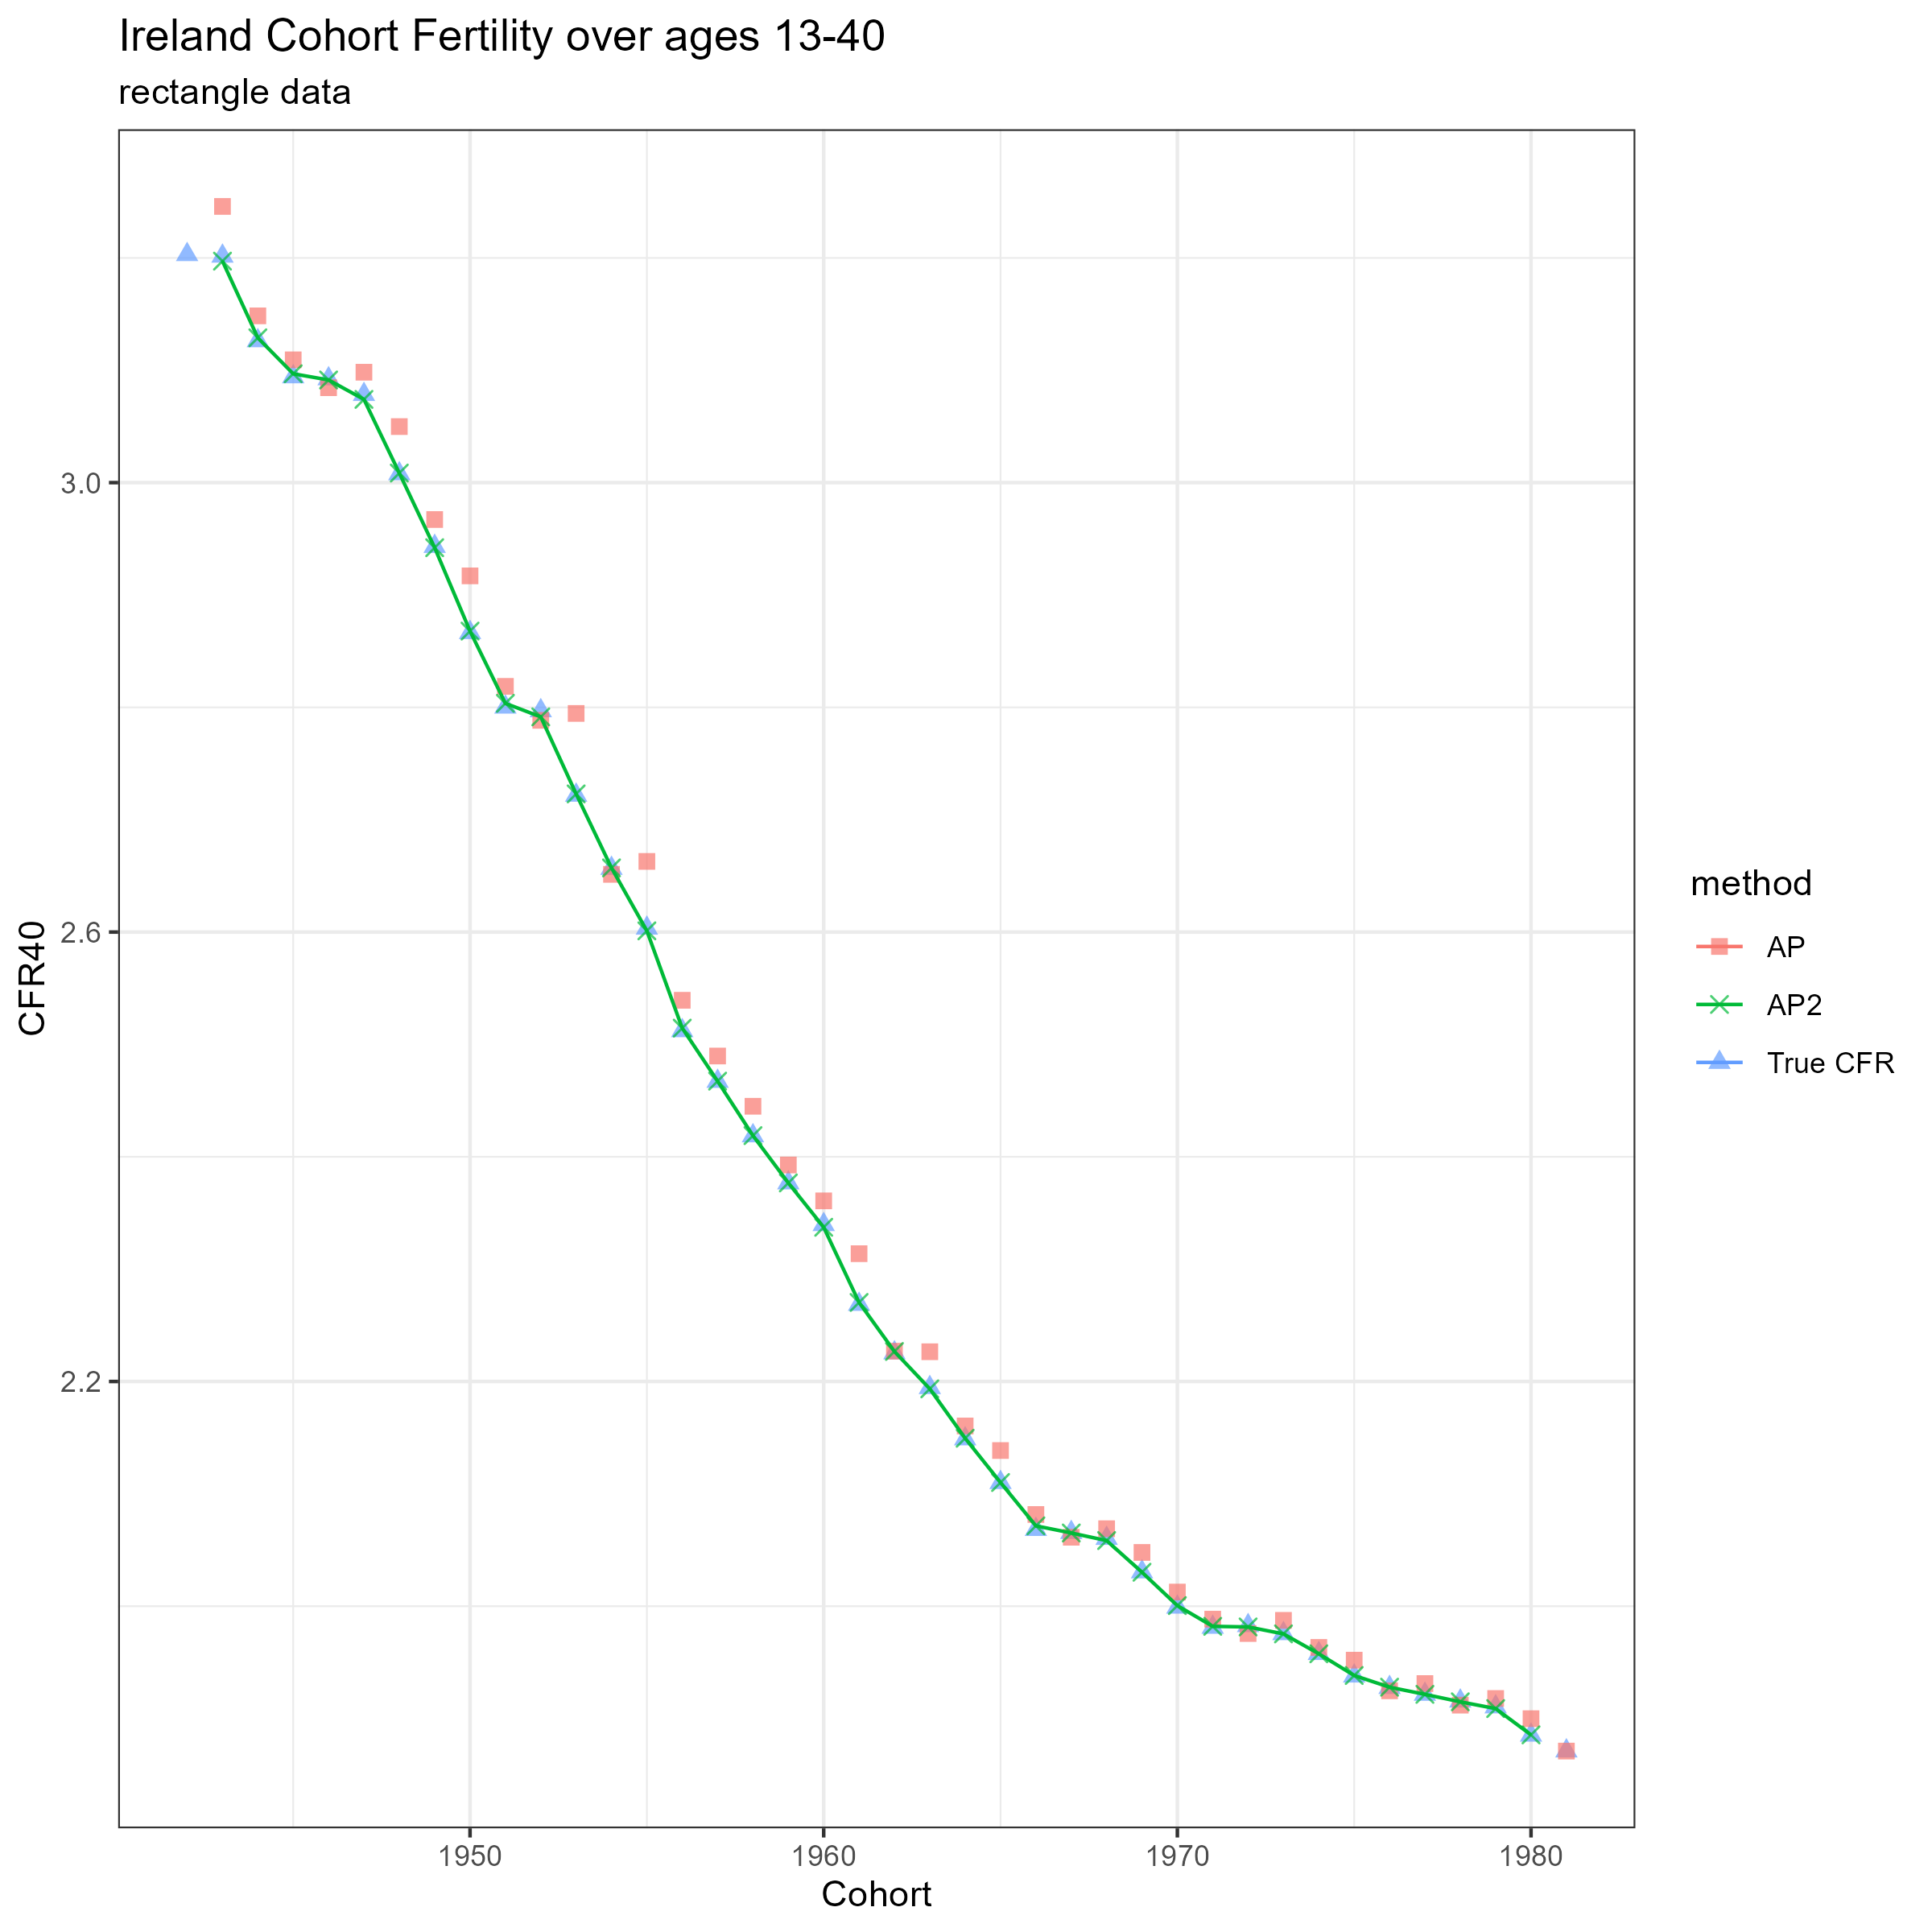
\includegraphics[width=0.9\textwidth]{Plots/IRL-CFR-levels}

\end{figure}

\begin{figure}
\caption{JPN \% err}

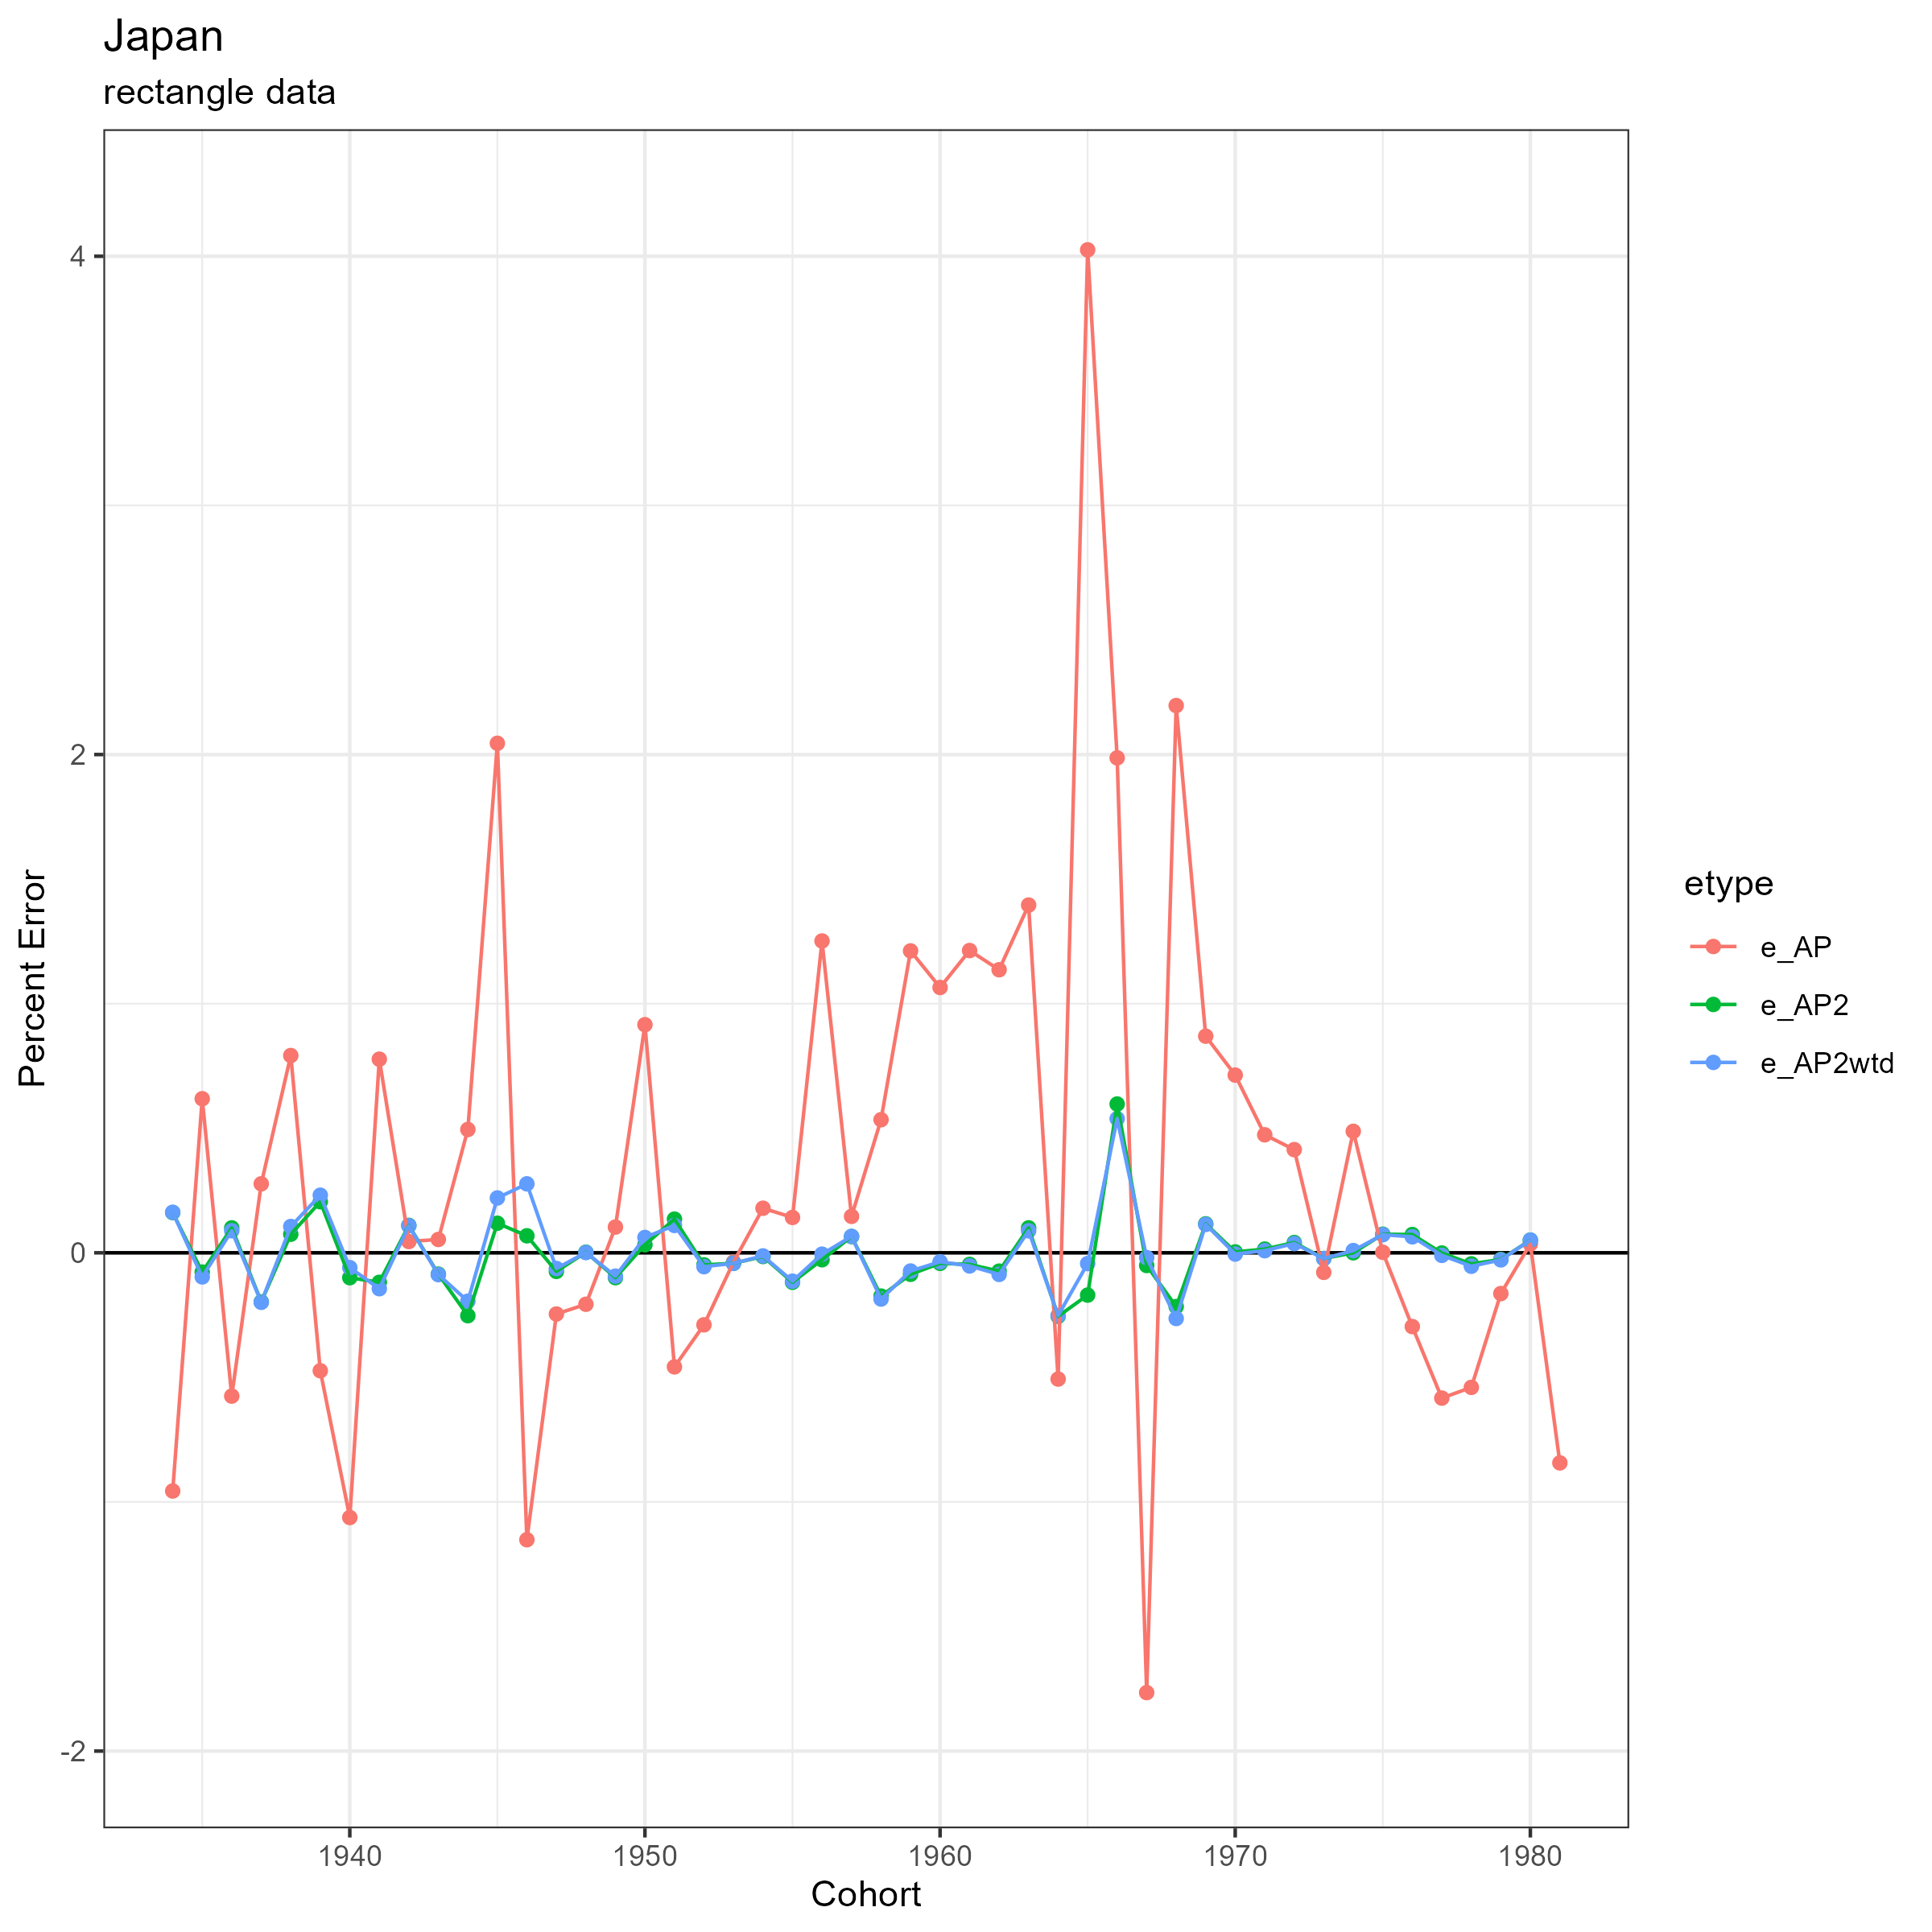
\includegraphics[width=0.9\textwidth]{Plots/JPN-CFR-errors}

\end{figure}

\end{document}
